\chapter{Sensing the Hand from the Wrist: EMG, Force Myography, and Bio-Acoustics}

Everything so far in this part of the book has been about motion. An accelerometer
feels the tug of gravity and the shove of acceleration; a gyroscope feels rotation;
a fused orientation estimate tells us how the forearm is tilted and turned in space.
That is genuinely useful, and we will lean on it hard. But the dream of a wrist-worn
musical controller -- playing notes by moving your fingers -- needs more than bulk
motion, and this chapter is where we find the channels that carry finger information
to the wrist.

\begin{focusbox}
Two facts frame this chapter, stated plainly before any math.

\textbf{Finger movement is detectable from a wrist or forearm band.} Curl a finger
and the tendon that drives it slides and the muscle that pulls it bulges, right there
under the strap. A force-myography (FMG) band feels that bulge; surface EMG taps the
electrical pulse that commands it. With a short per-finger calibration -- you perform
each movement a few times and the device records its signature -- live detection
becomes a matter of matching the current signal to your own calibrated templates.
This is achievable on buildable hardware.

\textbf{What the wrist cannot give you is continuous per-joint finger angles.} A
wrist-worn IMU alone cannot recover them, and neither can FMG or EMG: the full
$20$-dimensional hand pose is simply not present in wrist-surface signals. That target
needs sensors on the fingers themselves (rings). We will be clear about which side of
this line each goal falls on, because everything the instrument actually needs --
triggering notes by finger movement -- is on the doable side.
\end{focusbox}

The reason to confront this now, rather than at the capstone, is that the choice of
sensing modality reshapes \emph{everything} downstream: the sampling rate you need,
the filters you design, the features you extract, the per-finger calibration routine,
even the geometry of the band you strap on. The chapter lays out what each channel
senses, what it costs, how hard it is to build, and how a short calibration turns
each one into a finger detector.

\section{Why the wrist is a hard place to listen from}
\label{ch37:why-hard}

Hold your right wrist with your left hand and wiggle your fingers. Feel what moves.
The tendons that flex and extend your fingers run through the wrist like cables
through a conduit, and the muscles that pull those tendons sit mostly in the
\emph{forearm}, not the hand. The wrist is a privileged listening
post: a great deal of finger information passes through it. The work is reading the
\emph{form} that information takes by the time it reaches the surface.

\begin{intuitionbox}
Think of the forearm as a bundle of perhaps a dozen independent ropes (tendons),
each pulled by its own winch (muscle), all sheathed inside a flexible tube (skin,
fat, fascia). From outside the tube you are trying to figure out which ropes are
being pulled and how hard. An IMU is a sensor bolted to the \emph{outside of the
tube} that only feels the tube swinging around in space. It feels the whole tube
move; it is deaf to the ropes sliding inside. To hear the ropes you must press on
the tube (force myography), tap the electrical chatter of the winches (EMG), or
listen to the rumble the ropes make as they slide (bio-acoustics).
\end{intuitionbox}

This single picture organizes the whole chapter. Every modality below is a different
answer to ``how do I sense the ropes from outside the tube,'' and each answer trades
off cost, skill, robustness, and how much finger detail it actually recovers.

\subsection{Degrees of freedom: what you are trying to estimate}
\label{ch37:dof}

The human hand has roughly $21$ to $27$ kinematic degrees of freedom (DOF),
depending on how you count: four joints per finger reduced by tendon coupling, the
thumb's extra mobility, wrist flexion/extension and radial/ulnar deviation. A full
``hand pose'' is therefore a point in a space of about two dozen dimensions. That is
the target if you want to reconstruct the hand for, say, a virtual keyboard where
each finger is independent.

\begin{formalbox}
Let $\vec{q}(t)\in\R^{D}$ be the joint-angle vector, $D\approx 20$. A continuous
hand-tracking system estimates the full trajectory $\vec{q}(t)$. A gesture
detector instead reports only a \emph{label} $g(t)\in\set{1,\dots,K}$ from a
small set of $K$ movements -- finger~1 curled, finger~2 curled, pinch, rest -- plus
the moment of onset. These are different problems. The first is regression onto a
$20$-dimensional manifold; the second is deciding which of a handful of calibrated
patterns the current signal matches. The disappointment in this field comes from
quietly hoping a sensor that can do the second can do the first.
\end{formalbox}

Keep this distinction front of mind: \textbf{continuous pose} ($\vec{q}(t)$, hard,
wrist cannot do it) versus \textbf{discrete finger movement} ($g$, achievable from
the wrist with per-finger calibration). When we say ``the IMU cannot sense fingers,''
we mean it cannot do either from bulk motion. When we say ``FMG and EMG sense
fingers,'' we mean they reliably recover the discrete movement $g$ -- which finger
moved -- once the band has been calibrated to you.

\section{The IMU ceiling: what motion sensing alone can and cannot do}
\label{ch37:imu-ceiling}

Let us be precise about the wrist IMU rather than hand-waving. An IMU on the wrist
measures the linear acceleration and angular velocity of the wrist segment. By the
rigid-body kinematics of the previous chapters, that is exactly six numbers
describing the rigid motion of one bone-and-skin assembly. Finger flexion barely
moves the wrist segment; the tendons slide but the wrist bone's pose changes by an
amount swamped by ordinary tremor and the IMU's own noise floor.

\begin{whybox}
Why can't clever processing extract fingers from the IMU anyway? Because the
information is not there to extract. Mutual information cannot be created by a
filter. The map from finger pose to wrist-IMU output is many-to-one and nearly
constant: a huge range of finger configurations produce essentially the same
wrist-segment acceleration. No amount of FFT, wavelet, or signal conditioning can invert
a function that has thrown the input away. The IMU's blindness to fingers is an
information-theoretic fact about the sensor's placement, not a software shortcoming.
\end{whybox}

So what \emph{can} a wrist IMU do for the hand? Three things, each solid:

\begin{enumerate}
\item \textbf{Detect that a motion occurred.} A finger tap or a wrist flick produces
a transient acceleration spike. You can reliably detect the \emph{event}, even time
it to a millisecond, without knowing which finger.
\item \textbf{Classify a few coarse whole-hand or wrist gestures.} Wrist
flexion/extension, radial/ulnar deviation, supination/pronation, a sharp ``flick,''
a knock -- these move the wrist segment itself and are separable. Counts in the
literature are modest: a handful to a dozen gestures.
\item \textbf{Provide context and orientation} that other modalities lean on:
gravity direction, arm posture, gating ``is the hand even moving.''
\end{enumerate}

\begin{applicationbox}
The published wrist-IMU gesture literature backs up exactly these limits. A 2023
\emph{Sensors} (MDPI) study used a wrist IMU to \emph{count} finger and wrist
movements and detect their occurrence -- counting and detection, not pose recovery.
A 2020 \emph{PLOS One} study reached roughly $75$--$80\%$ accuracy on $14$ gestures,
but only by going \emph{multimodal}: an IMU \emph{plus} a contact
microphone (acoustic) on an Arduino DUE, not the IMU alone. The pattern across the
field is consistent: IMU-only systems handle a small gesture vocabulary; adding a
finger-driven channel -- acoustic, FMG, or EMG -- is what unlocks finger-level
distinctions. That is the edge our instrument will take: not one clever sensor, but
several modest ones fused.
\end{applicationbox}

\begin{figure}[H]
\centering
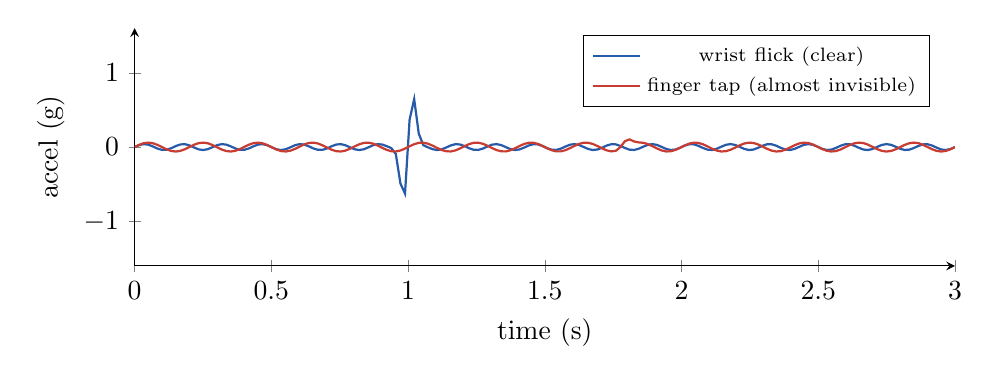
\begin{tikzpicture}
\begin{axis}[
  width=12cm, height=4.6cm,
  xlabel={time (s)}, ylabel={accel (g)},
  domain=0:3, samples=180,
  xmin=0, xmax=3, ymin=-1.6, ymax=1.6,
  axis lines=left, ytick={-1,0,1},
  enlargelimits=false, legend pos=north east, legend style={font=\scriptsize},
]
% a wrist flick: big transient near t=1.0
\addplot[sigblue, thick]
  {0.04*sin(deg(2*pi*7*x)) + 1.2*exp(-((x-1.0)^2)/0.0008)*sin(deg(2*pi*9*x))};
\addlegendentry{wrist flick (clear)}
% finger taps: tiny wiggles the IMU barely sees
\addplot[specred, thick]
  {0.06*sin(deg(2*pi*5*x)) + 0.10*exp(-((x-1.8)^2)/0.0006)};
\addlegendentry{finger tap (almost invisible)}
\end{axis}
\end{tikzpicture}
\caption{The IMU ceiling, drawn. A wrist flick (blue) drives a large, easily detected
transient. A finger tap (red) barely lifts the wrist accelerometer above its own
small-motion noise. The whole-hand event is legible; the finger event is not.}
\label{ch37:fig-imu-ceiling}
\end{figure}

\begin{goalbox}
For the wrist controller this fixes our architecture early. The IMU is the
\emph{conductor}, not the \emph{pianist}. It will give us arm orientation (which way
the hand points $\to$ pitch bend or instrument selection), motion gating (start/stop
of a phrase), and a few robust wrist gestures (octave up/down, mode switch). The
note-level finger triggering -- if we want fingers at all -- must come from a
different sensor on the band. Designing as if the IMU could do fingers is the single
most common way these projects fail.
\end{goalbox}

\section{Surface EMG: tapping the muscles' command lines}
\label{ch37:emg}

\begin{historybox}
\textbf{Galvani, Volta, and Du Bois-Reymond: The Birth of Electrophysiology}
The realization that muscles generate electricity began in the late 1780s in the laboratory of Italian physician Luigi Galvani at the University of Bologna. Galvani noticed that dissected frog legs twitched violently when suspended on brass hooks touching an iron railing during an electrical storm. Galvani concluded that living tissue contained an endogenous vital force: ``animal electricity'' stored like a Leyden jar in muscles and nerves.

Alessandro Volta fiercely disputed Galvani's theory, arguing that the twitch was merely a response to \emph{bimetallic contact electricity} generated by the junction of dissimilar metals (brass and iron) through moist salty frog tissue. Volta built the first chemical battery (the Voltaic pile) in 1800 to prove his contact theory, temporarily overshadowing Galvani's physiological claims.

The debate was definitively resolved in 1849 by German physician Emil du Bois-Reymond. Using an astatic galvanometer of extraordinary sensitivity (winding over three miles of fine insulated copper wire by hand to multiply magnetic deflection), du Bois-Reymond demonstrated that voluntary human muscle contraction generates genuine, endogenous electric currents, founding modern electrophysiology.
\end{historybox}

\begin{historybox}
\textbf{Otto Schmitt and the Differential Amplifier (1937)}
Even after du Bois-Reymond proved muscle action potentials existed, recording them non-invasively through surface electrodes on the human skin remained an engineering nightmare. A voluntary muscle contraction produces microvolt-scale potentials ($10\,\mu\text{V}$ to $1\,\text{mV}$) on the skin surface. But the human body acts as an efficient antenna picking up alternating magnetic and electric fields from $50/60\,\text{Hz}$ building power mains, which induce common-mode voltages of several volts across the body! A single-ended amplifier simply amplifies the deafening $60\,\text{Hz}$ wall buzz, completely drowning out the muscle signal.

In 1937, American biophysicist Otto Schmitt invented the \textbf{differential amplifier} (the cathode-coupled long-tailed pair) specifically to solve this biomedical obstacle. By measuring only the voltage difference across two adjacent electrodes ($V_+ - V_-$) while rejecting the voltage shared equally between them ($V_{\text{cm}}$), Schmitt achieved a high \textbf{Common-Mode Rejection Ratio} ($\text{CMRR} > 80\,\text{dB}$). Schmitt's differential architecture --- paired with the thresholding circuit that bears his name (the Schmitt trigger) --- made modern clinical electrocardiography (ECG) and surface electromyography (sEMG) physically possible.
\end{historybox}

\begin{trapbox}
\textbf{The Fatal Naive Pitfall: Motion Artifacts and the Skin-Electrode Double Layer}
Beginners building their first sEMG circuit often treat skin electrodes like simple multimeter probes touching copper wires. They plug in high-gain instrumentation amplifiers and are baffled when the signal wildly clips to the power rails whenever the wearer flexes a wrist or twitches an arm.

The culprit is the \textbf{electrochemical Helmholtz double layer}. Human stratum corneum (dry dead skin) has an electrical impedance of hundreds of kilo-ohms to several mega-ohms. When a metal electrode contacts skin electrolyte (perspiration or conductive gel), chemical half-cell reactions form a microscopic double layer of separated electric charges at the interface, creating an intrinsic DC potential of hundreds of millivolts.

When the arm moves, mechanical tension on the strap or electrode wire physically shears this charged double layer. This mechanical displacement modulates the half-cell capacitance, generating massive low-frequency voltage spikes ($0.5\,\text{Hz}$ to $20\,\text{Hz}$) measuring tens of millivolts --- \textbf{hundreds of times larger than the microvolt muscle action potentials!} 

A naive circuit without an aggressive analog high-pass filter ($f_c \approx 20\,\text{Hz}$) allows these motion artifacts to slam the differential amplifier into saturation, destroying all finger-gesture detection. Robust sEMG demands:
\begin{enumerate}
  \item Skin preparation (alcohol swabbing to reduce stratum corneum impedance).
  \item High-input-impedance instrumentation amplifiers ($>10^{10}\,\Omega$) to prevent voltage division losses.
  \item Active filtering: a sharp 2-pole high-pass above $20\,\text{Hz}$ to strip the double-layer motion artifact, alongside a $50/60\,\text{Hz}$ notch filter.
\end{enumerate}
\end{trapbox}

When your brain decides to flex a finger, motor neurons fire, and each firing makes a
patch of muscle fibers (a \emph{motor unit}) contract. Each contraction is preceded
by a tiny electrical depolarization that propagates along the fibers: the motor unit
action potential (MUAP). Surface electromyography (sEMG) places electrodes on the
skin over the forearm muscles and measures the summed electrical field of many motor
units firing -- the \emph{interference pattern}. It is, almost literally, an antenna
held over the muscle's command bus.

\begin{happeningbox}
What you are really recording in sEMG is not ``muscle force'' and certainly not
``finger angle.'' You are recording the superposition of many spiky action potentials,
each from a different motor unit, each firing at its own rate, low-pass filtered by
the tissue between the muscle and the skin. The raw signal looks like noise -- a
zero-mean, roughly symmetric, rapidly fluctuating waveform -- because it \emph{is} a
sum of many randomly-timed spikes. Its \emph{amplitude envelope} grows with how hard
and how many motor units are recruited. That envelope, not the raw wiggle, is what
carries the useful information.
\end{happeningbox}

\subsection{The signal and its spectrum}
\label{ch37:emg-signal}

Surface EMG is small and fast. Amplitudes are on the order of tens of microvolts to a
few millivolts. The useful energy spans roughly $20$ to $450$\,Hz, peaking around
$50$--$150$\,Hz. By the sampling theorem of the Nyquist chapter, you must sample above
twice the top frequency: $1000$\,Hz is a safe, common choice, $2000$\,Hz generous.

\begin{figure}[H]
\centering
\begin{tikzpicture}[font=\small, scale=0.88, every node/.style={transform shape}, >=Latex]
  \definecolor{sigblue}{RGB}{40,90,170}
  \definecolor{specred}{RGB}{200,60,50}
  \definecolor{targetgreen}{RGB}{62,145,95}
  \definecolor{quotientorange}{RGB}{214,127,35}
  \definecolor{structurepurple}{RGB}{120,88,165}

  % Time ruler at top
  \draw[->, gray!70] (0, 7.8) -- (13.5, 7.8) node[right, font=\footnotesize] {time $t$ (ms)};
  \foreach \x/\t in {0/0, 2.5/40, 5.0/80, 7.5/120, 10.0/160, 12.5/200} {
    \draw[gray!50] (\x, 7.7) -- (\x, 7.9);
    \node[gray!80, font=\tiny] at (\x, 8.1) {\t};
  }

  % Lane 1: Individual Motor Unit Action Potential (MUAP) Trains
  \begin{scope}[shift={(0,5.6)}]
    \node[anchor=east, font=\scriptsize\bfseries, align=right] at (-0.3, 0.9) 
      {Motor Unit 1\\Motor Unit 2\\Motor Unit 3};
    \draw[gray!30] (0,0) rectangle (12.5, 1.8);
    \node[font=\tiny, text=gray!80, anchor=north west] at (0.1, 1.75) {Neural Spikes \& MUAP Trains};

    \foreach \t in {1.25, 3.8, 6.4, 9.0, 11.6} {
      \draw[sigblue, thick] (\t-0.25, 1.3) -- (\t-0.08, 1.5) -- (\t, 1.05) -- (\t+0.08, 1.55) -- (\t+0.25, 1.3);
    }
    \draw[sigblue!40] (0, 1.3) -- (12.5, 1.3);

    \foreach \t in {2.0, 4.4, 6.8, 9.2, 11.4} {
      \draw[structurepurple, thick] (\t-0.25, 0.8) -- (\t-0.08, 0.98) -- (\t, 0.6) -- (\t+0.08, 1.02) -- (\t+0.25, 0.8);
    }
    \draw[structurepurple!40] (0, 0.8) -- (12.5, 0.8);

    \foreach \t in {2.8, 5.2, 7.6, 10.0} {
      \draw[quotientorange, thick] (\t-0.25, 0.3) -- (\t-0.08, 0.48) -- (\t, 0.12) -- (\t+0.08, 0.5) -- (\t+0.25, 0.3);
    }
    \draw[quotientorange!40] (0, 0.3) -- (12.5, 0.3);
  \end{scope}

  % Arrow 1 -> 2
  \draw[->, thick, gray!60] (6.25, 5.45) -- node[right, font=\tiny] {Asynchronous Superposition $\sum_i \text{MUAP}_i(t)$} (6.25, 4.85);

  % Lane 2: Raw sEMG Interference Pattern
  \begin{scope}[shift={(0,3.3)}]
    \node[anchor=east, font=\scriptsize\bfseries, align=right] at (-0.3, 0.6) {Raw sEMG\\Interference\\$x(t)$};
    \draw[gray!30] (0,0) rectangle (12.5, 1.4);
    \draw[gray!40, dashed] (0, 0.7) -- (12.5, 0.7);
    
    \draw[sigblue, thick] plot[domain=0:12.5, samples=150] 
      (\x, {0.7 + ( (\x > 2.0 && \x < 10.5) ? 0.5 : 0.08 ) * 
            ( 0.4*sin(\x*120) + 0.35*sin(\x*250) + 0.25*cos(\x*190) )});
    \node[font=\tiny, text=sigblue!80!black, anchor=north east] at (12.3, 1.35) {Contraction burst};
  \end{scope}

  % Arrow 2 -> 3
  \draw[->, thick, gray!60] (6.25, 3.15) -- node[right, font=\tiny] {Full-Wave Rectification $|x(t)|$} (6.25, 2.55);

  % Lane 3: Rectified EMG
  \begin{scope}[shift={(0,1.4)}]
    \node[anchor=east, font=\scriptsize\bfseries, align=right] at (-0.3, 0.5) {Rectified\\$|x(t)|$};
    \draw[gray!30] (0,0) rectangle (12.5, 1.0);
    \draw[specred, thick] plot[domain=0:12.5, samples=150] 
      (\x, {abs(( (\x > 2.0 && \x < 10.5) ? 0.55 : 0.08 ) * 
            ( 0.4*sin(\x*120) + 0.35*sin(\x*250) + 0.25*cos(\x*190) ))});
  \end{scope}

  % Arrow 3 -> 4
  \draw[->, thick, gray!60] (6.25, 1.25) -- node[right, font=\tiny] {Low-Pass Filter (Envelope Extraction)} (6.25, 0.65);

  % Lane 4: Linear Envelope (Muscle Activation)
  \begin{scope}[shift={(0,-0.3)}]
    \node[anchor=east, font=\scriptsize\bfseries, align=right] at (-0.3, 0.45) {Linear\\Envelope\\$e(t) \propto \text{Force}$};
    \draw[gray!30] (0,0) rectangle (12.5, 0.85);
    \fill[targetgreen!15] (0,0) -- plot[domain=0:12.5, samples=80] 
      (\x, {0.05 + 0.68*exp(-pow(\x - 6.25, 2)/6.5)}) -- (12.5, 0) -- cycle;
    \draw[targetgreen, very thick] plot[domain=0:12.5, samples=80] 
      (\x, {0.05 + 0.68*exp(-pow(\x - 6.25, 2)/6.5)});
    \node[font=\tiny, text=targetgreen!80!black, anchor=north east] at (12.3, 0.8) {Muscle activation / force};
  \end{scope}
\end{tikzpicture}
\caption{The physiological generation and signal-processing pipeline of surface EMG (sEMG). Top lane: spinal motor neurons asynchronously fire trains of action potentials across individual motor units (MUAPs). Second lane: the spatial and temporal summation of these potentials across skin-surface electrodes forms the zero-mean interference pattern $x(t)$. Third lane: full-wave rectification converts all fluctuations into positive power pulses $|x(t)|$. Bottom lane: low-pass filtering extracts the smooth linear envelope $e(t)$, which directly tracks physiological muscle activation and mechanical tendon tension.}
\label{ch37:fig-emg-pipeline}
\end{figure}


\begin{figure}[H]
\centering
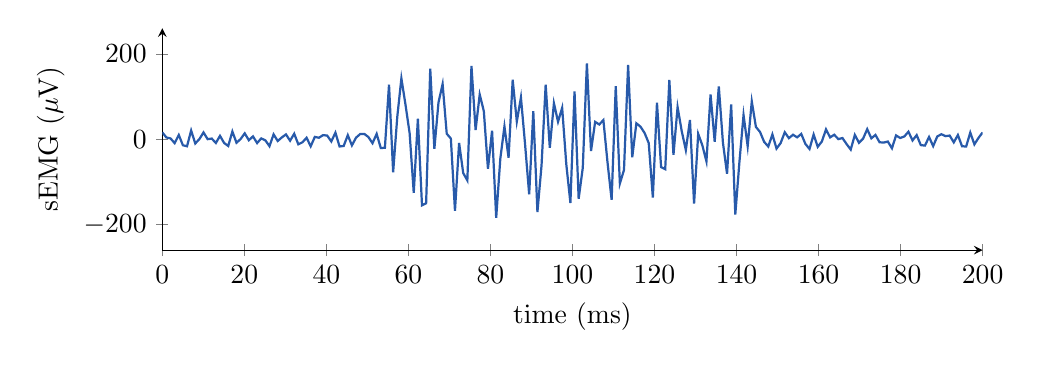
\begin{tikzpicture}
\begin{axis}[
  width=12cm, height=4.4cm,
  xlabel={time (ms)}, ylabel={sEMG ($\mu$V)},
  domain=0:200, samples=200,
  xmin=0, xmax=200, ymin=-260, ymax=260,
  axis lines=left, ytick={-200,0,200},
  enlargelimits=false,
]
% pseudo-random looking interference pattern with a contraction burst 55-145 ms
\addplot[sigblue, thick] {
  ( (x>55 && x<145) ? 1 : 0.12 ) *
  ( 90*sin(deg(2*pi*0.6*x)) + 70*sin(deg(2*pi*1.1*x+1))
    + 55*sin(deg(2*pi*1.7*x+2)) + 40*sin(deg(2*pi*2.3*x+0.5))
    + 30*sin(deg(2*pi*3.1*x+3)) )
};
\end{axis}
\end{tikzpicture}
\caption{A schematic sEMG trace: near-baseline chatter, then a contraction burst
(roughly $55$--$145$\,ms) where many motor units recruit and the amplitude envelope
swells. The information is in the envelope, not in any single oscillation.}
\label{ch37:fig-emg-trace}
\end{figure}

The signal-processing pipeline for sEMG is a textbook application of earlier chapters,
which is why it makes such a satisfying capstone modality:

\begin{enumerate}
\item \textbf{Band-pass filter}, roughly $20$--$450$\,Hz, to remove motion-artifact
drift below $20$\,Hz and high-frequency junk above the muscle band.
\item \textbf{Notch filter} at the mains frequency ($50$ or $60$\,Hz, plus harmonics)
to kill power-line pickup -- sEMG electrodes are excellent antennas for the wall.
\item \textbf{Rectify and smooth} to extract the amplitude envelope: take $\abs{x[n]}$
or $x[n]^2$, then low-pass. This is the ``linear envelope.''
\item \textbf{Feature extraction} per short window ($100$--$250$\,ms): mean absolute
value (MAV), root-mean-square (RMS), waveform length, zero crossings, and the
\emph{median frequency} of the spectrum (which drops as muscles fatigue).
\item \textbf{Match} the per-window feature vector against the per-finger templates
recorded during calibration -- nearest template, or a correlation/threshold test --
and emit the matching finger movement.
\end{enumerate}

\begin{formalbox}
Two of the workhorse features in closed form. For a window of $N$ samples,
\[
  \text{MAV} = \frac{1}{N}\sum_{n=1}^{N}\abs{x[n]},
  \qquad
  \text{RMS} = \sqrt{\frac{1}{N}\sum_{n=1}^{N} x[n]^2}.
\]
Both estimate the envelope amplitude. The \emph{median frequency} $f_{\mathrm{med}}$
is the frequency that splits the power spectrum into two equal halves:
$\sum_{f<f_{\mathrm{med}}} P(f) = \tfrac12 \sum_f P(f)$. It is prized because it
tracks muscle fatigue (the spectrum shifts toward lower frequencies as fast fibers
tire) while being insensitive to overall amplitude.
\end{formalbox}

\begin{connectionbox}
Notice how much of this is just the rest of the book reused. The band-pass and notch
are filter design (the filters chapter). The envelope is rectification followed by
low-pass -- a nonlinearity plus convolution. Median frequency is read straight off the
power spectral density from the spectral-estimation chapter. RMS is the
$\ell_2$ norm of the window divided by $\sqrt{N}$ -- the vector length from the
signals-as-vectors chapter. EMG is where the abstractions cash out.
\end{connectionbox}

\subsection{What EMG achieves -- and why calibration is indispensable}
\label{ch37:emg-perf}

Within a single session on a single person, with electrodes that have not moved,
sEMG finger detection is excellent: on a small set of finger movements (individual
finger flexions, a fist, a pinch) within-subject accuracy reaches roughly $99\%$.
That number is real, and it is exactly the regime our instrument runs in -- one user,
one strap-on, templates recorded minutes earlier. The catch is that the $99\%$ lives
on the \emph{near} side of calibration, not the far side.

\begin{trapbox}
The $99\%$ figure is a per-user, per-session number. Three effects explain why, and
each one points to the same fix -- calibrate to the wearer:
\begin{itemize}
\item \textbf{Cross-subject collapse.} Take templates built on my arm and apply them
to yours, and accuracy falls to $60$--$80\%$ or worse. Forearm anatomy, fat thickness,
and muscle geometry differ enough that one person's signatures do not fit another's.
The cure is not a bigger model -- it is a short enrollment on the actual wearer.
\item \textbf{Electrode-shift sensitivity.} Rotate the band a centimeter, or put it on
tomorrow, and the electrodes sit over different muscles. The templates from yesterday
no longer line up. A fresh $30$-second calibration on each donning restores it.
\item \textbf{Discrete, not continuous.} Detecting \emph{which} finger moved is the
solved, reliable part. Continuous, simultaneous, proportional angle of multiple
fingers from sEMG is still a research problem. Our instrument only needs the discrete
part, so this limit costs us nothing.
\end{itemize}
The lesson is not ``EMG is fragile.'' It is ``EMG is a per-user instrument'': measure
the wearer once, and it performs.
\end{trapbox}

\begin{historybox}
The state of the art lives in two recognizable places. The \emph{Myo armband}
(Thalmic Labs, $\sim 2014$) put eight dry sEMG electrodes plus an IMU on a consumer
band; it was discontinued but seeded a generation of student projects and datasets.
The \emph{MyoWare} board (an open, single-channel sEMG front-end from Advancer
Technologies / SparkFun) is the standard DIY entry point: it does the
instrumentation-amp, rectification, and envelope in analog, handing your Arduino a
clean envelope. At the high end, \emph{CTRL-labs} -- acquired by Meta in $2019$ --
pursued a high-density wrist sEMG band aiming at decoding individual motor-unit
activity, with the explicit ambition of typing and fine control from the wrist. Meta
has since publicly demonstrated a wrist sEMG wristband for neural input. The
trajectory is real. The cross-user, no-calibration version is not yet a commodity --
but the per-user, calibrate-then-play version, which is all we need, is squarely
within reach of a DIY build.
\end{historybox}

\begin{buildbox}
A minimal DIY sEMG channel:
\begin{itemize}
\item One \textbf{MyoWare 2.0} sensor (or a classic MyoWare) over a forearm flexor
belly, with the reference electrode on a bony, electrically-quiet spot (back of the
wrist, elbow).
\item Feed its \texttt{ENV} (envelope) output to an Arduino analog pin; or feed the
\texttt{RAW} output if you want to do your own band-pass/notch/rectify in software.
\item Sample RAW at $\geq 1000$\,Hz. The ENV pin is already low-frequency, so a few
hundred Hz suffices.
\item Expect to fight $50/60$\,Hz mains hum, motion artifacts when the wire tugs the
electrode, and sweat changing skin impedance over a session.
\end{itemize}
A tiny software pipeline on the RAW pin:
\end{buildbox}

\begin{lstlisting}[language=Python]
import numpy as np
from scipy.signal import butter, sosfilt, iirnotch, tf2sos

fs = 1000.0
# 20-450 Hz band-pass (forearm sEMG band)
bp = butter(4, [20, 450], btype="band", fs=fs, output="sos")
# 60 Hz mains notch (use 50 Hz in Europe)
b, a = iirnotch(60.0, Q=30.0, fs=fs)
notch = tf2sos(b, a)

def emg_envelope(raw, win=200):
    x = sosfilt(bp, raw)           # band-pass
    x = sosfilt(notch, x)          # remove mains hum
    x = np.abs(x)                  # rectify
    k = np.ones(win) / win         # moving-average smoother
    return np.convolve(x, k, mode="same")   # linear envelope

def mav(window):  return np.mean(np.abs(window))
def rms(window):  return np.sqrt(np.mean(window**2))
\end{lstlisting}

\begin{figure}[H]
\centering
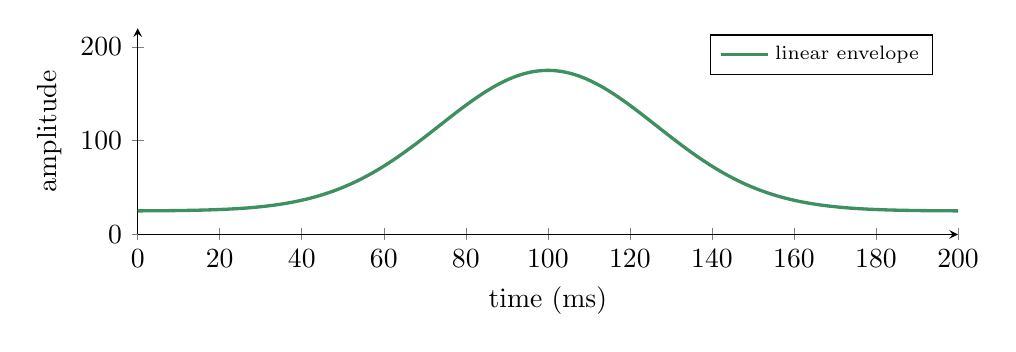
\begin{tikzpicture}
\begin{axis}[
  width=12cm, height=4.2cm,
  xlabel={time (ms)}, ylabel={amplitude},
  domain=0:200, samples=200,
  xmin=0, xmax=200, ymin=0, ymax=220,
  axis lines=left, ytick={0,100,200},
  enlargelimits=false, legend pos=north east, legend style={font=\scriptsize},
]
% rectified-and-smoothed envelope of the burst above
\addplot[targetgreen, very thick]
  {25 + 150*exp(-((x-100)^2)/1400)};
\addlegendentry{linear envelope}
\end{axis}
\end{tikzpicture}
\caption{The same contraction after rectify-and-smooth. The noisy interference
pattern of Figure~\ref{ch37:fig-emg-trace} becomes a clean amplitude bump whose height
and timing drive the template match. This is the curve a MyoWare ENV pin hands you in
hardware.}
\label{ch37:fig-emg-env}
\end{figure}

\section{Force myography: sensing the bulge, not the voltage}
\label{ch37:fmg}

There is a humbler modality that, for a DIY builder, is often the \emph{best} path to
finger sensing: force myography (FMG), sometimes called pressure myography. When a
forearm muscle contracts to pull a tendon, it changes shape -- it bulges. The
cross-section of the forearm physically deforms in a pattern that depends on which
muscles are active. FMG places a ring of force-sensitive resistors (FSRs) around the
wrist or forearm and measures how hard each one is being pushed.

\begin{intuitionbox}
EMG eavesdrops on the \emph{electrical command} to the muscle; FMG measures the
\emph{mechanical consequence}. Both ultimately report the same underlying event -- a
muscle contracting -- but through completely different physics. The mechanical
consequence is, refreshingly, easy to measure: a force-sensitive resistor is a few
cents, its signal is large and slow, and it does not care about your skin's electrical
impedance, your sweat, or the wall's $60$\,Hz hum. Where EMG is a delicate
microvolt antenna, FMG is a robust ``which buttons are being pushed'' band.
\end{intuitionbox}

\subsection{The signal: slow, large, robust}
\label{ch37:fmg-signal}

Each FSR is a resistor whose resistance drops as you press on it. Put it in a voltage
divider and you read a voltage that rises with force. Arrange $N$ of them in a band
and you get an $N$-dimensional vector $\vec{p}(t) = (p_1,\dots,p_N)$ -- a
\emph{pressure map} of the forearm's cross-section -- updated maybe $50$--$200$ times
a second. That is far slower than EMG's kilohertz, because muscle \emph{shape} changes
at the speed of movement, not at the speed of action potentials. Each finger movement
presses its own subset of the ring in its own pattern; per-finger calibration records
those patterns, and live detection reads which one is happening now.

\begin{figure}[H]
\centering
\begin{tikzpicture}
% a ring of 8 FSRs around a wrist cross-section, some pressed
\def\Rad{1.5}
\draw[gray!50, thick] (0,0) circle (\Rad);
\node[gray] at (0,0) {\scriptsize forearm};
\foreach \i/\lev/\pct in {0/0.9/90,1/0.2/30,2/0.15/25,3/0.7/75,4/0.85/85,5/0.1/20,6/0.1/20,7/0.3/40} {
  \pgfmathsetmacro{\ang}{\i*45}
  \pgfmathsetmacro{\xx}{(\Rad+0.18)*cos(\ang)}
  \pgfmathsetmacro{\yy}{(\Rad+0.18)*sin(\ang)}
  \pgfmathsetmacro{\sz}{0.10+0.30*\lev}
  \filldraw[draw=sourceblue, fill=sourceblue!\pct]
    (\xx,\yy) circle (\sz);
}
\node[sourceblue] at (0,-2.2) {\scriptsize 8 FSRs; darker/larger = more force};
\end{tikzpicture}
\caption{Force myography as a pressure map. A ring of force-sensitive resistors around
the forearm reads where the cross-section bulges. Different finger movements light up
different FSRs; calibration records each finger's pressure pattern, and live detection
matches the current pattern to the nearest recorded one.}
\label{ch37:fig-fmg-ring}
\end{figure}

\begin{whybox}
Why does such a crude sensor work for fingers when the IMU cannot? Because, unlike the
IMU, FMG \emph{is} downstream of the finger muscles. The bulge of the flexor
digitorum profundus when you curl your ring finger is a real, repeatable mechanical
signature at the forearm surface, and an FSR sitting over it sees a real change. The
IMU sits over the same skin but measures rigid-body motion, to which the bulge
contributes essentially nothing. Placement and physics, again, decide everything.
\end{whybox}

\begin{applicationbox}
The landmark DIY-scale result is \emph{WristFlex} (Dementyev and Paradiso, MIT Media
Lab, $2014$): a wristband of FSRs that classified about five pinch gestures at around
$80\%$ accuracy, at very low power, on hardware you could plausibly build. It is the
canonical demonstration that a cheap pressure band reads finger-level pinches the IMU
cannot. FMG has since been studied extensively for prosthesis control, often matching
or beating sEMG for robustness because it shrugs off sweat and electrode drift.
\end{applicationbox}

\begin{goalbox}
For our wrist instrument, FMG is the most realistic finger path. A band of $4$--$8$
FSRs distinguishes a set of pinches and finger curls -- enough to
trigger four or five different ``strings'' or drum pads -- once you have run the short
per-finger calibration that records each movement's pressure signature. Combined with
the IMU (orientation for pitch, motion for dynamics) this gives a playable
instrument without the microvolt fragility of EMG or the kernel-hacking of
bio-acoustics. If you build only one finger-sensing channel, build this one first.
\end{goalbox}

\begin{buildbox}
A starter FMG band:
\begin{itemize}
\item $4$ to $8$ FSRs (e.g. Interlink $402$) spaced evenly around an elastic wrist
strap, each in a voltage divider with a $\sim 10\,\text{k}\Omega$ resistor.
\item Read all channels on the microcontroller's ADC at $100$\,Hz; FMG bandwidth is
low, so this is generous.
\item Tighten the strap consistently -- preload sets the operating point of every FSR,
and a loose band is the FMG equivalent of EMG electrode shift.
\item Calibrate per session: guide the user through each target finger movement,
record a few seconds of each, and store the average pressure vector as that
movement's template. Live detection compares the current vector to the templates and
picks the nearest -- no training of any model, just measure-and-match.
\end{itemize}
\end{buildbox}

\begin{lstlisting}[language=Python]
import numpy as np

def read_fmg(adc, n=8):
    # raw 0..1 normalized FSR readings -> pressure vector
    return np.array([adc.read(ch) for ch in range(n)], dtype=float)

class NearestGesture:
    """Per-finger FMG matcher: store one template per movement, match nearest."""
    def __init__(self): self.templates = {}   # name -> mean pressure vector
    def enroll(self, name, samples):
        self.templates[name] = np.mean(samples, axis=0)
    def classify(self, p):
        best, bestd = None, np.inf
        for name, t in self.templates.items():
            d = np.linalg.norm(p - t)          # Euclidean distance in R^n
            if d < bestd: best, bestd = name, d
        return best
\end{lstlisting}

\begin{connectionbox}
The \texttt{NearestGesture} matcher is nothing but the inner-product / distance
geometry from the linear-algebra companion: each calibrated movement is a point in
$\R^{N}$, and detection is ``which template am I closest to.'' The robustness of FMG means
those points stay put across a session, so this geometric rule is not a placeholder
for something fancier -- it \emph{is} the method. Calibration records the templates;
detection measures a distance. No model is trained, and none is needed.
\end{connectionbox}

\section{Bio-acoustics: listening to the body's mechanical hum}
\label{ch37:bioacoustic}

There is a third, more exotic channel. When tendons slide, joints move, and fingers
tap, they generate mechanical vibrations -- structure-borne sound -- that propagate
through the arm. A sensitive accelerometer pressed to the skin, sampled fast enough,
becomes a \emph{contact microphone} for the body. This is bio-acoustic sensing.

\begin{happeningbox}
The trick that makes bio-acoustics work is a re-use of the accelerometer you already
have, but at a radically higher sample rate. Ordinary IMU use samples the
accelerometer at a few hundred Hz to track gross motion. If instead you read it at a
few kilohertz, it stops being a motion sensor and starts being a vibration sensor: it
hears the rumble of tendons, the click of a tap, the resonance of the bones. Different
finger actions excite the arm's mechanical structure differently, and those
differences live in the audio-band spectrum, not in the slow motion signal.
\end{happeningbox}

\begin{historybox}
The defining work is \emph{ViBand} (Laput, Xiao, Harrison, CMU, UIST $2016$). They
sampled a smartwatch accelerometer at $4000$\,Hz -- far above its normal use -- turning
it into a bio-acoustic microphone on the wrist. With it they recognized hand gestures,
distinguished objects being touched and even held power tools by their vibration
signature, and modulated data through the body. It shows what treating a motion
sensor as a frequency instrument buys you: the entire spectral toolkit of this book,
applied to a $4$\,kHz accelerometer stream.
\end{historybox}

\begin{trapbox}
Bio-acoustics is powerful but the hardest of these modalities to DIY, for a concrete
reason: getting a stock smartwatch or phone to deliver accelerometer samples at
$4$\,kHz usually requires \emph{modifying the device kernel or driver}, because
standard OS sensor APIs cap the rate far below that. The signal processing is
approachable; the plumbing to obtain the high-rate stream is not. On a dedicated
microcontroller wired directly to a high-bandwidth accelerometer (e.g. a $\geq
6$\,kHz-capable part read over SPI) you can hit the rate, but you are now doing
embedded engineering, not app development.
\end{trapbox}

\begin{goalbox}
This is why our build puts a dedicated microcontroller on the wrist instead of leaning
on a phone's sensors. A small wrist node wired to a high-bandwidth accelerometer over
SPI can read it at a few kilohertz, treating it as a contact/bio-acoustic channel for
taps and finger contacts -- alongside the same node's ordinary low-rate IMU motion and
the FMG ring. The node samples and lightly filters all three, then streams them over
BLE. The phone, which never had to hit $4$\,kHz itself, runs the calibration routine
and the deeper offline analysis. The hard ViBand plumbing problem dissolves once the
high-rate sensor lives on a chip you control rather than behind a locked OS API.
\end{goalbox}

\begin{figure}[H]
\centering
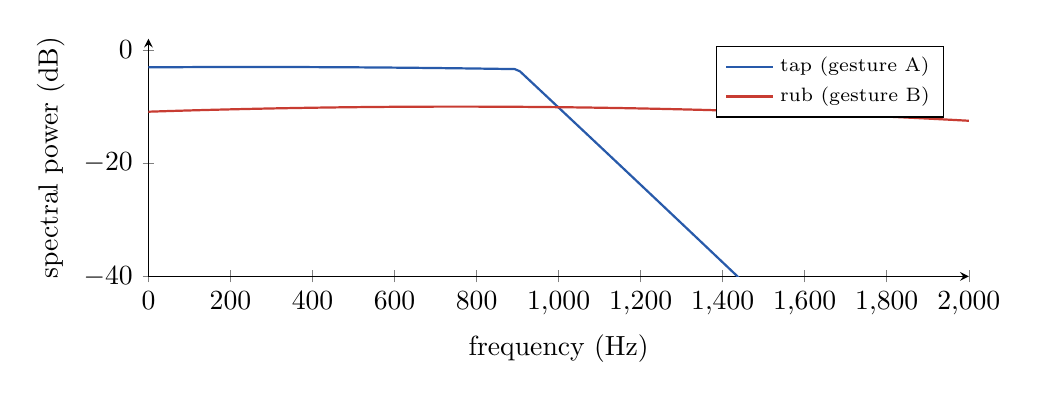
\begin{tikzpicture}
\begin{axis}[
  width=12cm, height=4.6cm,
  xlabel={frequency (Hz)}, ylabel={spectral power (dB)},
  domain=0:2000, samples=160,
  xmin=0, xmax=2000, ymin=-40, ymax=2,
  axis lines=left, ytick={-40,-20,0},
  enlargelimits=false, legend pos=north east, legend style={font=\scriptsize},
]
% gesture A: low-frequency resonance hump
\addplot[sigblue, thick] {
  -3 - 0.0000009*(x-250)^2 - 8*( x>900 ? (x-900)/120 : 0 )
};
\addlegendentry{tap (gesture A)}
% gesture B: a higher resonance peak
\addplot[specred, thick] {
  -10 - 0.0000016*(x-750)^2
};
\addlegendentry{rub (gesture B)}
\end{axis}
\end{tikzpicture}
\caption{Why high-rate vibration sensing separates gestures. Two finger actions excite
the arm's mechanics at different frequencies; their bio-acoustic spectra (schematic)
peak in different places. At $300$\,Hz IMU sampling these spectra would be invisible;
at $4$\,kHz they are easy to tell apart.}
\label{ch37:fig-bioacoustic-spec}
\end{figure}

\section{The decision table}
\label{ch37:decision}

Putting the five modalities side by side is the most useful single thing this chapter
can leave you with. Read it as ``what do I actually get, for what cost and skill, and
what does calibration buy me.''

\begin{center}
\renewcommand{\arraystretch}{1.35}
\begin{longtable}{p{2.2cm} p{3.0cm} p{2.4cm} p{2.2cm} p{2.6cm}}
\toprule
\textbf{Modality} & \textbf{What it senses} & \textbf{Finger detail} & \textbf{Cost / skill} & \textbf{Robustness} \\
\midrule
\endhead
Wrist IMU
 & Rigid motion of the wrist segment
 & None (continuous); a few coarse wrist/whole-hand gestures
 & Very low / low
 & High (just motion) \\
Surface EMG
 & Electrical command to forearm muscles
 & Good \emph{discrete} finger gestures; $\sim 99\%$ within-subject, much lower cross-subject
 & Medium / medium--high
 & Low: sweat, electrode shift, mains hum \\
Force myography
 & Mechanical bulge of muscles/tendons
 & Moderate: a few pinches/curls ($\sim 80\%$ on $5$, WristFlex)
 & Very low / low--medium
 & High: sweat-robust, no electrodes \\
Bio-acoustics
 & High-rate vibration (contact mic)
 & Good for taps/textures and some gestures (ViBand)
 & Medium / high (needs $\sim 4$\,kHz stream)
 & Medium: needs firm coupling, kernel access \\
Finger-worn IMUs (rings)
 & Motion/orientation of each finger directly
 & \emph{Continuous} pose, $\sim 9^{\circ}$ joint error
 & Medium / medium; not wrist-only
 & High, but intrusive (sensors on fingers) \\
\bottomrule
\end{longtable}
\end{center}

\begin{focusbox}
The single most important row is the last one. \textbf{Continuous finger pose --
the kind a virtual keyboard or full hand avatar needs -- requires sensors on the
fingers themselves}, typically small IMUs in rings, which report each finger's motion
directly and reach roughly $9^{\circ}$ of joint-angle error (the ``Learning on the
Rings'' line of work on finger-worn continuous tracking). No wrist-only modality
delivers this; the information is not in wrist-surface signals to begin with. What the
wrist modalities \emph{do} deliver -- once calibrated to the wearer -- is reliable
detection of \emph{which finger moved}, which is exactly what triggering notes
requires. The line to hold is narrow and clear: discrete finger movement from the
wrist, yes; continuous independent finger angles from the wrist, no.
\end{focusbox}

\subsection{A decision flow for the builder}
\label{ch37:decision-flow}

\begin{enumerate}
\item \textbf{Do you only need a few triggers and coarse wrist gestures?}
Wrist IMU alone. Cheap, robust, you already have it.
\item \textbf{Do you need to detect which finger moved, on a budget, surviving a
sweaty performance?} Force myography with per-finger calibration. Best DIY finger
path.
\item \textbf{Do you want the richest finger vocabulary and can run a $30$-second
calibration on each donning?} Surface EMG (start with MyoWare).
\item \textbf{Do you want tap/contact/texture sensing and can obtain a high-rate
accelerometer stream?} Bio-acoustics (ViBand-style), best as a fused channel on a
wrist node you control.
\item \textbf{Do you truly need continuous, independent finger angles?} Put sensors on
the fingers (rings). Accept that this is no longer a wrist-only device.
\end{enumerate}

\begin{aestheticbox}
The deeper lesson outlives the gesture controller. Sensing is choosing \emph{where to
stand} relative to the phenomenon, and signal processing only ever recovers what the
sensor's vantage point preserves. The IMU, EMG, FMG, and accelerometer-as-microphone
all watch the same hand; they differ entirely in which slice of reality reaches them.
Mastering DSP is partly mastering filters and transforms, but it begins with this
humbler, geometric question: from where I am standing, is the information I want even
present in the signal? If it is not, no transform will conjure it.
\end{aestheticbox}

\section{Combining modalities: the realistic capstone}
\label{ch37:fusion}

The literature's recurring answer -- and ours -- is \emph{fusion}. The IMU and a
finger-sensing channel are complementary: the IMU is robust and cheap but finger-blind;
FMG and EMG see fingers but need per-finger calibration. Together they cover each
other's weaknesses. Recall that the PLOS One $14$-gesture result only reached its
$75$--$80\%$ by combining IMU with acoustic sensing; neither alone did as well. Our
edge over the single-modality lab papers is exactly this: a high-rate IMU, an FMG/FSR
ring, and a high-rate accelerometer used as a contact sensor, all fused, all
calibrated to the wearer -- not a cleverer model on one sensor.

\begin{goalbox}
Our capstone architecture, which the final chapter will build, splits cleanly into a
thin wrist node and a phone (Figure~\ref{ch37:fig-architecture}):
\begin{itemize}
\item \textbf{IMU} (the conductor): orientation $\to$ pitch / pitch-bend; motion energy
$\to$ note velocity / dynamics; a few wrist gestures $\to$ mode and octave switches;
motion gating $\to$ note-on/note-off windows.
\item \textbf{FMG band} (the fingers): $4$--$8$ FSRs $\to$ a set of pinches/curls
that select which ``string'' or pad fires, resolved by matching the live pressure
vector to the per-finger templates from calibration. Chosen over EMG for
sweat-robustness and DIY simplicity; EMG is the upgrade path for a richer vocabulary,
finger-worn rings the upgrade path for continuous angles.
\item \textbf{Wrist node}: samples all sensors (including the high-rate accelerometer
as a contact channel), applies light filtering, compresses, and BLE-streams. A
lightweight on-device template-match handles the low-latency live-play path.
\item \textbf{Phone}: runs the guided per-finger calibration, builds the templates and
thresholds, conditions the streamed signals, and does deeper offline analysis from the
logged data. No model is trained -- the method is measure-and-match throughout.
\end{itemize}
This is buildable, musically expressive, and clear about its limits -- it triggers
notes from detected finger movements and never pretends to read finger joint angles it
cannot read.
\end{goalbox}

\begin{figure}[H]
\centering
\begin{tikzpicture}[
  font=\scriptsize,
  box/.style={draw, rounded corners=2pt, align=center, inner sep=3pt, minimum height=8mm},
  sens/.style={box, fill=blue!6},
  node1/.style={box, fill=orange!8},
  phone/.style={box, fill=green!7},
  >={Stealth[length=2mm]},
]
% sensors
\node[sens] (imu)  at (0,2.2)  {IMU\\(motion)};
\node[sens] (fmg)  at (0,1.1)  {FMG ring\\(pressure)};
\node[sens] (acc)  at (0,0)    {hi-rate accel\\(contact)};
% wrist node
\node[node1] (node) at (3.6,1.1) {Wrist node\\sample + light filter\\compress + BLE\\live template-match};
% phone
\node[phone] (phone) at (8.0,1.7) {Phone\\guided calibration\\build templates\\condition + offline analysis};
\node[box, fill=gray!8] (midi) at (8.0,0.2) {MIDI out\\note / chord / CC};
\draw[->] (imu) -- (node);
\draw[->] (fmg) -- (node);
\draw[->] (acc) -- (node);
\draw[->] ([yshift=2mm]node.east) -- node[above, sloped]{BLE stream} ([yshift=2mm]phone.west);
\draw[->] ([yshift=-2mm]phone.west) -- node[below, sloped]{templates} ([yshift=-2mm]node.east);
\draw[->] (node) |- (midi);
\end{tikzpicture}
\caption{The capstone split. The thin wrist node samples three sensors, filters lightly,
and BLE-streams to the phone; the phone runs the guided per-finger calibration and
offline analysis and pushes templates back. A lightweight on-node template match drives
the low-latency MIDI path. No model is trained anywhere -- calibration measures
templates, detection matches them.}
\label{ch37:fig-architecture}
\end{figure}

\begin{recoverybox}
If you remember one diagram from this chapter, make it the ``ropes in a tube'': the
IMU feels the tube swing, FMG presses the tube, EMG taps the winches, bio-acoustics
hears the ropes slide, and only sensors on the ropes themselves read continuous
finger pose. Everything else here is detail hung on that picture.
\end{recoverybox}

\section{Capabilities, Limitations, and the Road Ahead}
\label{ch37:capabilities-limits}

\subsection{What Forearm Muscle Sensing Unlocked}
Tapping into muscle electrical commands (sEMG), tendon radial expansion (FMG), and mechanical shear transients (bioacoustics) overcomes the rigid kinematic ceiling of inertial sensors:
\begin{itemize}
  \item \emph{Non-invasive finger intent from the wrist:} Without donning gloves, rings, or optical cameras, a wristband can detect discrete finger movements (pinching thumb, index curl, fist clench, finger spread) by reading the forearm musculature.
  \item \emph{Multi-modal synergy:} Fusing FMG (low-frequency static pressure for sustained grips) with sEMG (instantaneous electrical motor activation for trigger timing) and high-rate bioacoustics (transient shockwaves from finger taps) produces robust, highly responsive input for real-time controllers.
  \item \emph{Direct calibration without machine learning:} Because tendon geometries are repeatable within a single wear session, a 30-second guided enrollment records template signatures that can be classified deterministically with simple Euclidean distance or cross-correlation.
\end{itemize}

\subsection{Honest Downsides and Inherent Limitations}
Bio-signal sensing is notoriously volatile:
\begin{itemize}
  \item \emph{The 20-DOF kinematic impossibility:} The forearm contains deep and superficial muscle layers sliding over each other. Many distinct finger configurations project to nearly identical surface electrical or pressure distributions. Reconstructing continuous, independent joint angles for all twenty knuckles from a wristband remains underdetermined.
  \item \emph{Wrist pose cross-talk:} The flexor and extensor muscle bellies shift physically when the wrist itself rotates or flexes. An index-finger pinch performed with the wrist bent upward creates a dramatically different FMG/EMG spatial pattern than the same pinch performed with the wrist straight.
  \item \emph{Physiological non-stationarity:} Sweating alters skin impedance dynamically; muscle fatigue shifts the sEMG power spectrum toward lower frequencies; and taking the band off and putting it back on shifts electrode locations by millimeters, requiring recalibration.
\end{itemize}

\subsection{The Road Ahead: From Static Signatures to Dynamic Trajectories}
Whether we record inertial angular rates, muscle action potential envelopes, or force-myography pressure vectors, real gestures are not static snapshots: they are \textbf{dynamic paths that unfold over time}. A user may flick a wrist or tap a finger slowly or quickly. In \textbf{Chapter 38}, we tackle temporal gesture recognition, introducing \textbf{Dynamic Time Warping (DTW)} to warp and align elastic time-series, alongside windowed feature extraction to turn streaming waveforms into reliable musical events.

\section{Exercises}
\label{ch37:exercises}

\begin{exercise}
Explain, in terms of mutual information and the map from finger pose to sensor output,
why no amount of filtering or processing can make a wrist IMU
recover individual finger joint angles. What property of the pose-to-output map is the
real obstacle?
\end{exercise}

\begin{exercise}
sEMG has useful energy up to about $450$\,Hz. State the minimum sampling rate required
by the Nyquist criterion, justify why $1000$\,Hz is a common safe choice, and explain
what specifically goes wrong (in the spectrum) if you sample the RAW sEMG at $400$\,Hz.
\end{exercise}

\begin{exercise}
Given a one-second sEMG window sampled at $1000$\,Hz, write the formulas for MAV and
RMS, and argue from the definition of the $\ell_2$ norm why
$\text{RMS} = \norm{\vec{x}}_2 / \sqrt{N}$. For a window of constant amplitude $A$
(a square wave), compute both MAV and RMS.
\end{exercise}

\begin{exercise}
The median frequency $f_{\mathrm{med}}$ splits the power spectrum into equal halves.
Suppose a muscle fatigues and its spectrum shifts uniformly downward by $15\%$. What
happens to $f_{\mathrm{med}}$, and why is it a better fatigue indicator than total
power (RMS)?
\end{exercise}

\begin{exercise}
Force myography reads a pressure vector $\vec{p}\in\R^{8}$. During calibration you
record one template per finger movement by averaging samples. Explain geometrically
why nearest-template matching works, and describe one realistic situation (hint: strap
tension) that shifts all eight readings and breaks it. How would you make the matcher
robust to that shift?
\end{exercise}

\begin{exercise}
Contrast EMG and FMG at the level of physics: both ultimately report ``a muscle
contracted,'' yet one is a microvolt electrical signal and the other a slow large
mechanical one. List two consequences of this difference for the sampling rate, and
two for real-world robustness.
\end{exercise}

\begin{exercise}
ViBand samples a wrist accelerometer at $4000$\,Hz. Compute its Nyquist frequency.
Explain why the \emph{same} accelerometer sampled at $200$\,Hz cannot distinguish two
gestures whose bio-acoustic signatures differ only above $300$\,Hz, referencing the
spectra in Figure~\ref{ch37:fig-bioacoustic-spec}.
\end{exercise}

\begin{exercise}
Using the decision table of Section~\ref{ch37:decision}, choose a sensing modality for
each of these targets and justify it in one sentence: (a) a fist/open-hand toggle for
a simple game; (b) a sweat-proof five-pinch live-performance trigger; (c) a research
prototype distinguishing $20$ finger gestures within one session; (d) a full
hand-avatar with independent finger motion.
\end{exercise}

\begin{exercise}
The PLOS One study reached $75$--$80\%$ on $14$ gestures only by fusing IMU with
acoustic sensing. Propose a fused feature vector for an IMU+FMG template matcher (list
at least three IMU-derived and three FMG-derived features), and explain which gestures
each modality is expected to disambiguate.
\end{exercise}

\begin{exercise}
Sketch (in prose or a block diagram) the full capstone pipeline from the goalbox in
Section~\ref{ch37:fusion}: which sensor produces which MIDI message, where filtering
happens, where windowing happens, where calibration builds the templates, and where
the live template match sits. Mark which steps run on the wrist node and which on the
phone. Identify the one place where an overclaim about sensor limits would most likely
creep in, and how your design avoids it.
\end{exercise}
